\documentclass[11pt]{article}
%\usepackage{amsfonts}
\usepackage{amsmath}
\usepackage{fancybox}%,times}
\usepackage{graphicx,psfrag,epsf}
%\usepackage{amsmath}
\usepackage{enumerate}
\usepackage{graphicx,psfrag}
\usepackage{multirow}
\usepackage{epsfig}
%\usepackage{rotating}
\usepackage{subfigure}
\usepackage{theorem}
\usepackage{natbib,psfrag}
\usepackage{tikz}
\usepackage{xcolor}
\usepackage{kotex}
\newcommand{\blind}{0}
\usepackage{graphicx}
\DeclareGraphicsExtensions{.pdf,.png,.jpg}

\addtolength{\oddsidemargin}{-.75in}%
\addtolength{\evensidemargin}{-.75in}%
\addtolength{\textwidth}{1.5in}%
\addtolength{\textheight}{1.3in}%
%\addtolength{\topmargin}{-.6in}%
\addtolength{\topmargin}{-.8in}%

%\theoremstyle{break}
\newtheorem{The}{Theorem}
\newtheorem{Def}{Definition}
\newtheorem{Pro}{Proposition}
\newtheorem{Lem}{Lemma}
\newtheorem{Cor}{Corollary}
\newtheorem{asp}{Assumption}


\renewcommand{\thefootnote}{\arabic{footnote}}
%\renewcommand{\thefootnote}{\alph{footnote}}
%\renewcommand{\thefootnote}{\roman{footnote}}
%\renewcommand{\thefootnote}{\fnsymbol{footnote}}

\begin{document}


%\bibliographystyle{natbib}

\newcommand{\Ito}{$It\hat{o}$'$s~Lemma$}

\newcommand\ind{\stackrel{\rm ind}{\sim}}
\newcommand\iid{\stackrel{\rm iid}{\sim}}
\renewcommand\c{\mathbf{c}}
\newcommand\y{\mathbf{y}}
\newcommand\z{\mathbf{z}}
\renewcommand\P{\mathbf{P}}
\newcommand\W{\mathbf{W}}
\newcommand\X{\mathbf{X}}
\newcommand\Y{\mathbf{Y}}
\newcommand\Z{\mathbf{Z}}
\newcommand\J{{\cal J}}
\newcommand\B{{\cal B}}
\newcommand\K{{\cal K}}
\newcommand\N{{\rm N}}
\newcommand\bs{\boldsymbol}
\newcommand\bth{\bs\theta}
\newcommand\bbe{\bs\beta}
\renewcommand\*{^\star}

\def\spacingset#1{\renewcommand{\baselinestretch}%
{#1}\small\normalsize} \spacingset{1}


%%%%%%%%%%%%%%%%%%%%%%%%%%%%%%%%%%%%%%%%%%%%%%%%%%%%%%%%%%%%%%%%%%%%%%%%%%%%%%

  \bigskip
  \bigskip
  \bigskip
  \begin{center}
    {\LARGE\bf April 18, 2019 }
  \end{center}
  \medskip

%\begin{abstract}
%\end{abstract}

%\noindent%
%{\it Key Words:}  AECM algorithm; Astrophysical data analysis;
%ECME algorithm; Incompatible Gibbs sampler; Marginal data
%augmentation; Multiple imputation; Spectral analysis

\spacingset{1.45}


\section{False Discovery Rate}
\begin{figure}[h]
	\centering
	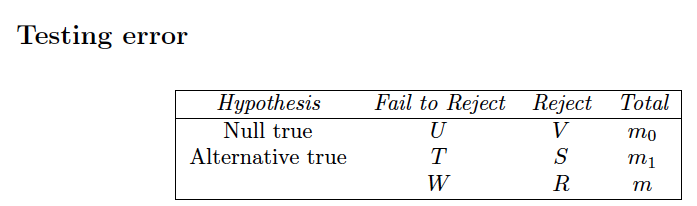
\includegraphics[width=0.7\linewidth]{fdr}
	\caption{Testing Error}
	\label{fig:fdr}
\end{figure}
$Q$ is The proportion of the rejected null hypothesis which are erroneously rejected
\begin{align*}
Q = \frac{V}{R} = \frac{V}{V+S} \;, \; FDR = E[Q] = E[\frac{V}{R}]
\end{align*}
\begin{itemize}
	\item Useful approach to simultaneous testing
	\item relies on $p$-values that is on null hypothesis areas
\end{itemize}
\section{Local FDR}
\begin{align*}
\text{Null Hypothesis : }& H_1 , H2, \dots , H_i, \dots, H_N \\
\text{Test Statistics : }& z_1, z_2, \dots , z_i , \dots, z_N
\end{align*}
We assume that th N cases are divided into two classes, null or non-null, occurring with prior probabilities $p_0$ or $p_1 = 1- p_0$ and density of test statistic $z$ depending upon its class.
\begin{align*}
p_0 = Pr\{null\}& \; f_0(z) \text{density if null}\\
p_1 = Pr\{non-null\}& \; f_1(z) \text{density if non-null}
\end{align*}
We can write the null subdensity as,
\begin{align*}
f_0^+(z) = p_0 f_0(z)
\end{align*}
and the mixture density
\begin{align*}
f(z) = p_0 f_0(z) + p_1 f_1(z)
\end{align*}
by definition the local false discovery rate is,
\begin{align*}
fdr(z) &\equiv Pr\{null | z\} = p_0 f_0(z) / f(z)\\
&=f_0^+(z)/f(z)
\end{align*}
Letting the $F_0(z)$ and $F_1(z)$ be the cdf's define $F_0^+ = p_0 F_0(z)$ and $F(z) = p_0 F_0(z) + p_1 F_1(z)$
\begin{align*}
Fdr(z) &\equiv Pr\{null |Z \le z\} = p_0 F_0(z) / F(z)\\
Fdr(z) &= \int_{-\infty}^{z} fdr(Z)f(Z)dZ/\; \int_{-\infty}^{z} f(Z)dZ\\
&=E_f \{ fdr(Z)  |Z \le z \}
\end{align*}
$Fdr(z)$ is the average of $fdr(z)$ for $ Z \le z$, $Fdr(z)$ will be less than $fdr(z)$ in the usual situation where $fdr(z)$ decreases as $|z|$ gets large.

\section{Example}
\begin{align*}
Y_i | \beta_i&  \stackrel{ind}{\sim}N(\beta_i,1)\\
\beta_i& \sim \begin{cases} 0 &\text{with probability 0.8} \\
N(0,1) &\text{with probability 0.2} \end{cases} \\
\end{align*}
We can write $Y_i = \beta_i + \epsilon_i$, where $\epsilon_i \sim N(-,1)$
\begin{itemize}
	\item $p_0 = Pr\{null\} = 0.8$
	\item $p_1 = Pr\{non-null\} = 0.2$
	\item $f_0(y) \sim N(0,1)$ density of $Y_i$ if null
	\item $f_1(y) \sim N(0,2)$ density of $Y_i$ if non-null
	\item $f(y) = p_0 f_0(y) + p_1 f_1(y)$
\end{itemize}
Local FDR is
\begin{align*}
fdr(y) &= p_0 f_0(y) / f(y) = Pr\{null | Y_i = y\}\\
&=Pr(\beta_i = 0 | Y) = \frac{0.8 \cdot N(0,1)}{0.8 \cdot N(0,1) + 0.2 \cdot N(0,2)}
\end{align*}
For instance $fdr(0) = \frac{0.8 \cdot f_0(0)}{0.8 \cdot f_0(0) + 0.2 \cdot f_1(0)} = 0.8888889 $

\begin{figure}[h]
	\centering
	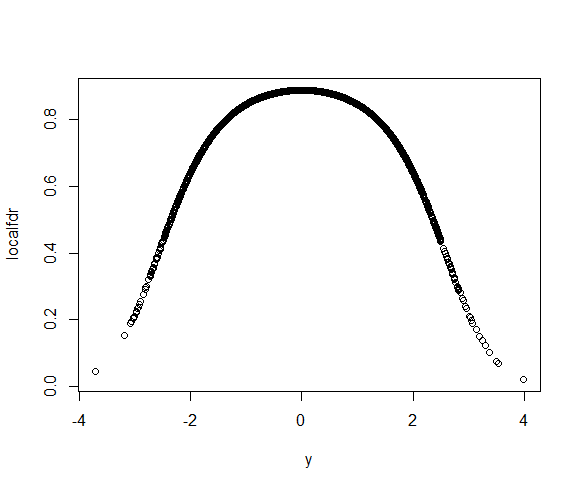
\includegraphics[width=0.7\linewidth]{Rplot02}
	\caption{N = 10000}
	\label{fig:rplot}
\end{figure}

\end{document}
